\section{Spectra}
\subsection{Correcting to the rest frame}
\label{sec:spec_restframe}
Correcting the observed wavelength for the relativistic Doppler effect is done by: 
\begin{equation}
    \lambda_{rest \,\, frame} = \frac{\lambda_{observed}}{1+z_{helio}}.
\end{equation}
Correcting the observed flux is similar: 
\begin{equation}
    f_{rest \,\, frame} = \frac{f_{observed}}{(1+z_{helio})^{2}}.
\end{equation}

Why? Because redshift affects wavelength, it also affects frequency, i.e., photon energy. You get a two-fold effect here---one factor of $(1 + z)$ is from the wavelength increasing, and the other is from the intensity decreasing. 

\subsection{Normalizing to a particular $z$}
Sometimes, you want your spectrum flux as if it were at some redshift $z_{ref}$ that you've chosen. Do not use the rest frame spectrum for this calculation. First thing's first, you need the luminosity distance to your object.

\begin{equation}
    D_{L} = (1+z_{helio})D_{M},
\end{equation}
where $z_{helio}$ is the actual redshift for your object, and $D_{M}$ is the comoving transverse distance. In Python, you can use \texttt{astropy.cosmology}'s function \texttt{comoving\_transverse\_distance}, which takes $z_{CMB}$ as its input (so you'll also need your object's RA and dec), to calculate $D_{M}$. If we assume an FLRW universe, then our cosmological scale factor is $a(t) = 1/(1+z)$. Then,
\begin{equation}
    \frac{a(t_{ref})}{a(t_{actual})} = \Big( \frac{1 + z_{helio}}{1+z_{ref}} \Big) \Big( \frac{D_{L, actual}}{D_{L, ref}} \Big)^{2}
\end{equation}

Finally, convert your flux by using this value:
\begin{equation}
    F_{ref} = F_{actual}\Big( \frac{1 + z_{helio}}{1+z_{ref}} \Big) \Big( \frac{D_{L, actual}}{D_{L, ref}} \Big)^{2} = F_{actual} \Big(\frac{a(t_{ref})}{a(t_{actual})} \Big)
\end{equation}

\subsection{Absorption lines}
\subsubsection{Pseudo-equivalent width}
Pseudo-equivalent width (pEW) is a measure of the strength of an absorption line. It combines the depth and the width of the line into one measurement by integrating over the feature. There's a really good run-down of pEW in \cite{Galbany2015}. So, we're going to borrow from them. Figure~\ref{fig:pew} shows an absorption feature. You start with one like the one on the left (red). We want to measure the strength of the absorption feature, but the problem with SNe is that there are so many absorption and emission lines and there's doppler shift everywhere, so we don't really know where the continuum is. \textit{But}, we need a way to fairly compare absorption features between different SNe, which means removing the continuum. So, we make a ``pseudo-continuum'' to approximate a small region of the actual continuum. Lines are nice, so all you do to make the pseudo-continuum is draw a line across the top of the absorption feature. We remove the ``continuum'' by normalizing the absorption feature to the pseudo-continuum. You only do this for the one feature---for each absorption feature, you need a new pseudo-continuum. After you've normalized to the pseudo-continuum, you end up with the \textit{right} panel of Figure~\ref{fig:pew} (green). Now, you can measure the area and fairly compare line strengths between SNe. 

\begin{figure}[h!]
    \centering
    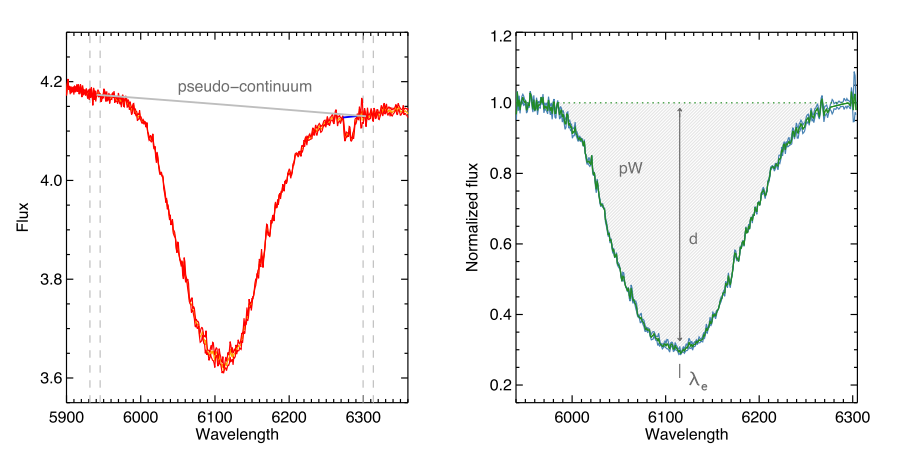
\includegraphics[width=0.9\textwidth]{figs/Screenshot from 2022-07-12 16-05-37.png}
    \caption{\textit{Left}: Un-normalized absorption feature. \textit{Right}: The same absorption feature normalized to the pseudo-continuum marked on the \textit{left}. $d$ is the feature depth and $\lambda_{e}$ is the center wavelength. The shaded area is the pEW (pW in the figure). Figure from \cite{Galbany2015}.}
    \label{fig:pew}
\end{figure}

That's great and all, but how do we actually do all this in practice? There are a lot of ways. Let's break it down into steps and talk about 'em. This is \textit{not} an exhaustive list, nor is it the only way to do this---these are merely suggestions. Let your imagination run free, spectral padawan.

\begin{enumerate}
    \item \textbf{Finding the pseudo-continuum:} The challenging part of this step is avoiding noise. We don't want an unrealistic pseudo-continuum because we picked a point where there's a statistical spike or dip in the measurement. You can smooth the data with a moving average, or use the Savitzky-Golay filter from \texttt{scipy.signal.savgol\_filter()}. Discussing the differences between these two is outside the scope of this manual, but you should always understand the techniques you're using! 
    \item \textbf{Normalizing to the pseudo-continuum:} Take your smoothed flux and divide by the line you drew. Here's some Python-inspired pseudo-code to help you out:
    \begin{minted}[
    bgcolor=lightgray,
    frame=leftline,
    framesep=-3mm]
    {python}
    continuum = scipy.interpolate.interp1d(flux[start_point],
        flux[end_point])
    normalized_flux = flux[start_point:end_point]
        /continuum(wavelength[start_point:end_point])
    \end{minted}
    
    \item \textbf{Integrating over the absorption feature:} You can do this via summation directly over the normalized data or by fitting a Gaussian and integrating that. 
\end{enumerate}

Now... we weren't going to have this entire discussion without talking about error on pEW, of course. The error for this kind of ``guesstimation'' thing is hard to quantify precisely, so I recommend a bootstrapping method like the one in \cite{Galbany2015}. Instead of choosing fixed endpoints for your pseudo-continuum, draw randomly from some small region around your chosen endpoints $N$ times to get $N$ sets of different, but all reasonable, endpoints. Now, calculate the pEW as discussed above for each set of endpoints. Then, your final pEW measurement is the mean of all $N$ measurements, with the standard deviation of all $N$ measurements as your error on pEW. 

\subsubsection{Ejecta velocity}
\label{sec:ejectavelocity}

\subsection{Synthetic photometry}

If you're here, you're wondering how to make photometry from some spectra. In short, this is obtained by integrating under the spectrum in the region covered by a given filter. 

The area under the spectrum, $F$, in a given filter $X$, is calculated by
\begin{equation}
    F_{X} = \int_{\lambda_{1}}^{\lambda_{2}} \lambda f(\lambda) R_{X}(\lambda) d\lambda,
\label{eqn:synthint}
\end{equation}

%%%PUT IN A PLOT OF WHAT RESPONSE FUNCTIONS LOOK LIKE, OVERLAYED ON A SPECTRUM

where $f(\lambda)$ is your spectrum, and $R_{X}(\lambda)$ is your filter. The $\lambda$ term is in there if we're using photon-counting detectors. If you're using an energy-counting detector, you would drop this, i.e., your integrand is $f(\lambda) R_{X}(\lambda) d\lambda$.

However, we can't often use the continuous version of this function with our data. So, we discretize it:

\begin{equation}
    F_{X} = \sum_{i=\lambda_{1}}^{\lambda_{2}} \lambda_{i} f(\lambda_{i}) R_{X}(\lambda_{i})(\lambda_{i} - \lambda_{i-1}),
\label{eqn:synth_discrete}
\end{equation}

where $f(\lambda_{i})$ is the energy flux at a particular wavelength $\lambda_{i}$, and $R_{X}(\lambda_{i})$ is the response function for the filter at wavelength $\lambda_{i}$. We're using a discretized version of an integral, so $(\lambda_{i} - \lambda_{i-1})$ is the same as $d\lambda$. From now on, this chapter will be written as if we are using Equation \ref{eqn:synth_discrete}.

Then, for a photon-counting detector, the variance of $F$ (using Equation \ref{eqn:errorprop}) is:

\begin{equation}
    \sigma_{F}^{2} = \sum_{i=\lambda_{1}}^{\lambda_{2}} \lambda_{i}^{2}\sigma_{f(\lambda_{i})}^{2} R_{X}(\lambda_{i})^{2}(\lambda_{i} - \lambda_{i-1})^{2}
\end{equation}

For an energy-counting detector, the variance of $F$ is:
\begin{equation}
    \sigma_{F}^{2} = \sum_{i=\lambda_{1}}^{\lambda_{2}} \sigma_{f(\lambda_{i})}^{2} R_{X}(\lambda_{i})^{2}(\lambda_{i} - \lambda_{i-1})^{2}
\end{equation}

Individual magnitudes are calculated by
\begin{equation}
    m = -2.5\log_{10}\Big(\frac{F}{F_{ref}}\Big) = -2.5\log_{10}(F) + 2.5\log_{10}(F_{ref}) = -2.5\log_{10}(F) - m_{ref}.
\end{equation}
\textit{Wait---what are $F_{ref}$ and $m_{ref}$}? Good question. Because magnitudes are inherently relative quantities, we need to use some reference object to convert flux into magnitudes. You can get reference objects from \href{https://www.stsci.edu/hst/instrumentation/reference-data-for-calibration-and-tools/astronomical-catalogs/calspec}{CALSPEC}. Photometric systems are, unfortunately, out of the scope of this manual at this time. Let's say we're using the Vega system, with the star Vega (Alpha Lyrae) from now on. 

This means we need to use Equation \ref{eqn:synth_discrete} on our reference object, Vega to calculate $F_{ref}$. You'll use the \textit{same} response function as you use for your supernova spectrum. This means that $m_{ref}$ is the... reference magnitude? What does THAT mean? If magnitudes are inherently relative quantities, do we then compare our reference object to something \textit{else}? A valid concern, but no! This is called a \textit{zero point}. For the Vega system, astronomers have defined the magnitude of the star Vega such that the $m_{Vega}$ = 0 in all bands. So, if you're using the Vega system, $m_{ref}$ is probably just 0 (unless some literature tells you otherwise, which is possible, so make sure you're familiar with the photometric system and filters you're using).

So anyway, the variance of $m$ (for an energy-counting detector) is:
\begin{equation}
    \sigma_{m}^{2} = \frac{\partial m}{\partial f}^{2} \sigma_{f}^{2} = \frac{\partial m}{\partial F}^{2} \Big( \sum_{i=\lambda_{1}}^{\lambda_{2}} \frac{\partial F}{\partial f(\lambda_{i})} \sigma_{f(\lambda_{i})}\Big)^{2} = \Big( \frac{-2.5}{F\ln10} \Big)^{2} \sum_{i=\lambda_{1}}^{\lambda_{2}}\sigma_{f(\lambda_{i})}^{2} R_{X}(\lambda_{i})^{2}(\lambda_{i}-\lambda_{i-1})^{2}
    \label{eqn:m_err}
\end{equation}

Note that the summation term on the right-hand side of the equation is the same as $\sigma_{F}^{2}$. 

If you're looking for \textit{colors}, I've got your back there, too. For arbitrary color $X-Y$,
\begin{equation}
    m_{X} - m_{Y} = -2.5\log \Big( \frac{F_{X}}{F_{ref,X}} \Big) + 2.5\log \Big( \frac{F_{Y}}{F_{ref,Y}} \Big)
\end{equation}.
We can propagate the error here, too. If you want, you can assume $X$ and $Y$ are independent, and do $\sigma_{X-Y} = \sqrt{\sigma_{X}^{2} + \sigma_{Y}^{2}}$. However, we can be more rigorous and not assume independence. We're going to use $\sigma^{2} = \mathbf{JCJ^{T}}$---the explanation of this formula is beyond the scope of this manual. $\mathbf{J}$ is the Jacobian of your spectrum (remember, your spectrum is a function!), and $\mathbf{C}$ is its covariance matrix. The following method will work \textit{if you have an error for the flux in your data spectrum}.

For ease of calculations, we will treat $m_{X}-m_{Y}$ as a function of $f(\lambda_{i})$ (our supernova spectrum, in discrete wavelength chunks). Then, for arbitrary color $X-Y$, the Jacobian is:
\begin{equation}
\label{eqn:jac2}
\mathbf{J}_{X-Y} = 
\begin{bmatrix}
    
        \frac{\partial m_{X-Y}}{\partial f(\lambda_{0})} & \frac{\partial m_{X-Y}}{\partial f (\lambda_{1})} & \dots & \frac{\partial m_{X-Y}}{\partial f(\lambda_{N})} \\
    
\end{bmatrix}
\end{equation}

\parindent = 0 mm

where $N$ is the last measured wavelength in the spectrum. The $i$th entry is: 
\begin{equation}
    \frac{\partial m_{X-Y}}{\partial f(\lambda_{i})} = -\frac{1.09}{F_{X}} R_{X}(\lambda_{i})(\lambda_{i}-\lambda_{i-1}) + \frac{1.09}{F_{Y}}R_{Y}(\lambda_{i})(\lambda_{i}-\lambda_{i-1})
\end{equation}

Then, the covariance matrix is diagonal, and each entry is the spectrum error provided in the data:
\begin{equation}\mathbf{C_{X-Y}} = 
    \begin{bmatrix}
        \sigma_{f(\lambda_{0})}^{2} &  & & \\
         & \sigma_{f(\lambda_{1})}^{2}&  & \\
         &  & \ddots &  \\
        & & & & \sigma_{f(\lambda_{N})}^{2}\\
    \end{bmatrix}.
    \label{eqn:cov}
\end{equation}
Now, we use $\sigma^{2} = \mathbf{JCJ^{T}}$, and boom, we have color error without assuming independence for the filters. 

\subsection{Things to watch out for}
\subsubsection{Response function units}
Your response function will likely be normalized, but may be given in either normalized flux units or normalized photon counts. You need to know which units you have. If you need the other, don't fret---you can convert it to the other unit system. Let's say you have a response function in normalized photon units, but your spectrum is in energy flux units (ergs/cm$^{2}$/s/$\mathrm{\AA}$). It's best to convert the spectrum to photons. For each $i$th wavelength, you do:

\begin{equation}
    f_{\gamma}(\lambda_{i}) = f_{E}(\lambda_{i})\frac{\lambda_{i}}{hc},
\end{equation}
where $h \approx 6.626 \times 10^{-27}$ ergs $\cdot$ s and $c \approx 3\times 10^{18}$ is the speed of light in $\mathrm{\AA}$/s. 

Why convert the spectrum instead of the response function? Well, CCDs count photons, so it's ideal to do as much as possible in these units. 

\subsubsection{Help! My results are unreasonable!}

Did you check all of the following:
\begin{itemize}
    \item Did you convert both your standard spectrum \textit{and} your data spectrum from ergs to photons (or vice versa)?
    \item When you converted between ergs and photons, did you use the correct units for the constants? Remember, for ergs/cm$^{2}$/s/$\mathrm{\AA}$, use $h \approx 6.626 \times 10^{-27}$ ergs $\cdot$ s and $c \approx 3\times 10^{18}$ $\mathrm{\AA}$/s. 
    \item When you converted between ergs and photons, did you multiply by the conversion factor when you should have divided (or vice versa)? 
    \item Does the wavelength range of your filter fall completely inside the wavelength range of your spectrum? 
\end{itemize}

\subsection{Step-by-step Explain Like I'm 5}